\documentclass[a4paper, 11pt]{article}
\usepackage[english]{babel}
\usepackage[utf8]{inputenc}
\usepackage{amsmath}
\usepackage{graphicx}
\usepackage{float}
\usepackage{fixltx2e}
\usepackage{listings}
\usepackage{color}
\usepackage{latexsym}
\usepackage{lstautogobble}
\usepackage[colorinlistoftodos]{todonotes}
\usepackage[margin=3cm]{geometry}
\usepackage{hyperref}
\usepackage{libertine}
\usepackage{tikz}
\hypersetup{
	hidelinks, 
	colorlinks = true,
	linkcolor = black,
}

\usetikzlibrary{shapes, arrows}

\newtheorem{definit}{Definizione}[subsection]

\begin{document}
	\clearpage
	\begin{titlepage}
		\centering
		\vspace*{\fill}
		{\scshape\LARGE Università degli Studi di Verona \par}
		\vspace{1.5cm}
		\line(1,0){150} \\
		{\huge\bfseries Crittografia\par}
		\line(1,0){150} \\
		\vspace{0.5cm}
		{\scshape\Large Riassunto dei principali argomenti\par}
		\vspace{2cm}
		{\Large\itshape Davide Bianchi\par}
		\vspace{1cm}
		\vspace{5cm}
		\vspace*{\fill}
		% Bottom of the page
		{\large \today\par}
	\end{titlepage}
	\thispagestyle{empty}
	\newpage
	\tableofcontents
	\newpage
	
	\section{Introduzione}
	Iniziamo dando alcune definizioni fondamentali. Si useranno i termini \textit{ciphertext} e \textit{plaintext} per indicare rispettivamente il testo cifrato e quello in chiaro.
	
	\begin{definit}[Crittografia]
		Insieme dei metodi per rendere un messaggio non leggibile ad altri.
	\end{definit}
	
	\begin{definit}[Steganografia]
		Insieme dei metodi per nascondere l'esistenza di un messaggio in un altro contenuto.
	\end{definit}
	
	\begin{definit}[Crittoanalisi]
		Analisi del ciphertext per ottenere il plaintext corrispondente.
	\end{definit}
	
	\begin{definit}[Bit]
		Conoscenza di un evento che ha probabilità $0.5$ di verificarsi. Da ciò si ricava che \[ I = -log_2P \]
	\end{definit}
	
	Un generico sistema crittografico è strutturato come: \\
	
	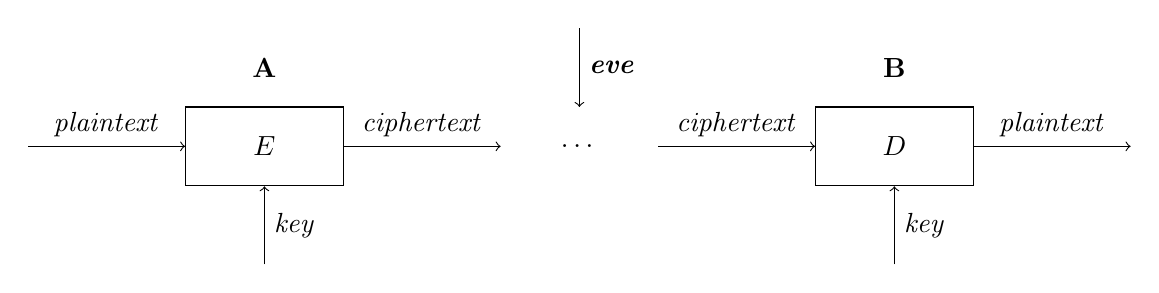
\begin{tikzpicture}
		\node at (4,0) [rectangle,draw, minimum width=2cm, minimum height=1cm] (E) {$E$};
		\draw (E);
		\draw[->] (1,0) -- (E) node[above, midway] {\textit{plaintext}};
		\draw[->] (4,-1.5) -- (E) node[right, midway] {\textit{key}};
		\draw[->] (E) -- (7,0) node[above, midway] {\textit{ciphertext}};
		\node at (8,0) (dots) {$\dots$};
		\node at (12,0) [rectangle,draw, minimum width=2cm, minimum height=1cm] (D) {$D$};
		\draw[->] (9,0) -- (D) node[above, midway] {\textit{ciphertext}};
		\draw[->] (12,-1.5) -- (D) node[right, midway] {\textit{key}};
		\draw[->] (D) -- (15,0) node[above, midway] {\textit{plaintext}};
		\node at (4,1) {\textbf{A}};
		\node at (12,1) {\textbf{B}};
		\draw[->] (8, 1.5) -- (8,0.5) node[right, midway] {\textbf{\textit{eve}}};
	\end{tikzpicture}
	
	dove:\begin{itemize}
		\item \textbf{A} e \textbf{B} sono i due enti che si devono scambiare il messaggio cifrato;
		\item \textbf{\textit{eve}} è un terzo che tenta di decrittare il messaggio;
		\item $E$ e $D$ sono i sistemi di \textit{encrypt} e \textit{decrypt};
		\item i 3 punti ($\dots$) rappresentano il mezzo impiegato per la trasmissione del messaggio (qualunque esso sia).
	\end{itemize}
	
	Ovviamente, per \textit{eve}, che tenta di decrittare il messaggio, non ha senso tentare di insistere se il costo della decrittazione è maggiore del valore dell'informazione da proteggere. In tal senso il sistema di cifratura è "sicuro". 
	
	La funzione $E$, inoltre, per essere sufficientemente affidabile, deve essere invertibile (in caso contrario non si potrebbe decrittare il messaggio), ma deve essere difficile fare ciò (in tal caso si dice che $E$ è una \textit{one-way function}). Con la chiave la funzione diventa facile anche da invertire (\textit{one-way trapdoor}). \newpage
	
	\section{Cifrari storici}
	\subsection{Cifrario di Cesare}
	Il messaggio viene cifrato sostituendo ogni lettera $l$ del messaggio con la $l+k$ esima lettera dell'alfabeto; la chiave quindi è data dalla coppia $(l, l+k)$. 
	
	Il cifrario di Cesare è facile da attaccare in quanto basta un attacco \textit{bruteforce}, quindi è sufficiente provare tutte le combinazioni (che sono in totale 26).
	
	\subsection{Permutazione casuale}
	Supponiamo di usare come cifrario una permutazione casuale dell'alfabeto, ovvero sostituendo ad ogni lettera dell'alfabeto un'altra lettera, in modo totalmente casuale. In tal caso l'attacco bruteforce richiederebbe tempo eccessivo (ci sono $26!$ pssibili combinazioni da provare, che sono decisamente troppe). 
	
	La tecnica usata per attaccare questo tipo di crittografia è l'\textit{analisi delle frequenze}, ovvero l'analisi delle lettere che capitano di più in una data lingua, e associare la lettera del messaggio cifrato con una data frequenza con quella nella lingua del messaggio con una frequenza simile.
	
	\subsection{Cifrario a coppie di lettere}
	Supponiamo di avere come chiave la parola \textit{MONARCHY}. Generiamo una tabella $5 x 5$, che viene riempita inserendo la chiave prima e poi le altre lettere dell'alfabeto in ordine, escludendo le lettere della chiave. \\
	
	\begin{center}
		\begin{tabular}{|c|c|c|c|c|}
			\hline
			M &O &N &A &R\\[1pt]
			\hline
			C &H &Y &B &D\\[1pt]
			\hline
			E &F &G &I/J &K\\[1pt]
			\hline
			L &P &Q &S &T\\[1pt]
			\hline
			U &V &W &X &Z\\[1pt]
			\hline
		\end{tabular} 
	\end{center}
	
	Per iniziare è necessario dividere il plaintext in coppie di lettere.
	Per codificare una lettera ci si sposta lungo la riga fino ad incolonnarsi sotto l'altra lettera della coppia. La lettera del ciphertext sarà quella in cui ci si trova.
	
	Attaccare il cifrario è semplice: è sufficiente analizzare le frequenze di coppie di lettere, anche se è leggermente più complesso che analizzare le singole lettere.
	
	\subsection{Cifrario di Vigenère}
	Il cifrario di Vigenère riprende l'idea del cifrario di Cesare. L'idea è la seguente: presa una chiave (es. \textit{key}), si ripete la chiave tante volte quanto è lungo il testo (eventualmente troncando l'ultima ripetizione), e si codifica la lettera con il corrispondete cifrario di Cesare. \\
	
	\noindent
	K E Y K E Y K E Y K E Y \\
	P R O V A D I T E S T O \\
	
	
	La prima lettera del cipher text sarà la lettera ottenuta dal cifrario di Cesare di chiave $(K,P)$, la seconda con la chiave $(E, R)$ e così via.
	
	Anche questo cifrario è semplice da attaccare, si parte dalla divisione del ciphertext in gruppi di lunghezza pari a quella della chiave, e si esegue l'analisi delle frequenze su ogni gruppo.
	
	\subsection{Enigma}
	Consideriamo ora la rappresentazione binaria di un cifrario di Cesare. Esistono solamente due chiavi possibili: \[ (0,1); (0,0) \]
	
	Consideriamo quindi un semplice esempio, con $K=0011, P=0101$. Applicando Vigenère otteniamo che $ C=0110$. Si può notare che, date $K_i$ una qualsiasi lettera della chiave e $P_i$ una qualsiasi lettera del plaintext, $C_i = K_i \oplus P_i$. Pertanto si può dedurre che $C=K\oplus P$. Vale in maniera analoga anche $P=K \oplus C$.
	
	È stato già verificato che il cifrario di Vigenère sia semplice da attaccare, ma se $|K| = |P|$ allora non è più applicabile la crittoanalisi data per il cifrario di Vigenère. 
	
	Tuttavia, se vale $|K| = |P|$, allora significa che la chiave è sostanzialmente una sequenza di bit casuali. In tal caso il ciphertext non avrebbe \textit{nessuna} relazione con il plaintext, e non sarebbe possibile ricavare alcuna informazione utile. Il problema di questo metodo sta nel fatto che ogni chiave è utilizzabile una sola volta, in caso contrario sarebbe possibile ricavare informazioni dai vari ciphertext ottenuti con la stessa chiave. (si parla in questo caso di \textit{one-time pad})
	
	La macchina Enigma (usata dai tedeschi nella II G.M.) usava questo metodo: cambiando chiave ogni giorno garantiva ciphertext difficilissimi da decifrare. Infatti generava una sequenza di permutazioni per una lettera, poi ruotava una permutazione, poi quella successiva e coosì via per ogni lettera.
	
	Ciò che rese decifrabili le comunicazioni generate da questa macchina fu il fatto che ogni messaggio iniziasse con la stessa sequenza di caratteri (un saluto ad Hitler).
	
	\section{Verso la crittografia moderna}
	
	
	
\end{document}